\chapter{  Luminometer system description}




%%%%%%%%%%%%%%%%%%%%%%%%%%%%%%%%%%%%%%%%%%%%%%%%%%%%%%%%%%%%%%%%%%%%%%%%%%%%%%%%%%%%%%%%%
\section{Pixel Clusters and the PCC method}

Luminosity measurements at CMS are provided by the several luminometers in the detector.
Each luminometer measures the event rate by reading out a specific quantity of objects observed by the detector, These can be for example clusters, coincidences or tracks. For the TEPX luminometers these objects are pixel clusters and coincidences, using the pixel cluster counting (PCC) method to provide offline luminosity measurements. This method was one of the main source of luminosity measurements for CMS, during the 2016-2018 data taking period, and it is expected to be the same for the Phase-2 upgrade.\\
The clustering algorithm is very complex, but striping it down to the most simple example: the algorithm considers a cluster of pixels only if two hits, or more,  activate neighboring pixels horizontally, vertically or diagonally, within the same module. Figure\ref{pixclust} shows an example of this.
\begin{figure}[H]
\begin{minipage}[b]{0.5\linewidth}
\centering
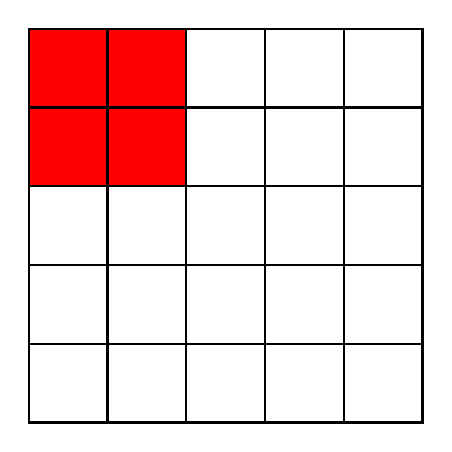
\begin{tikzpicture}
    [%%%%%%%%%%%%%%%%%%%%%%%%%%%%%%
        box/.style={rectangle,draw=black,thick, minimum size=1cm},
    ]%%%%%%%%%%%%%%%%%%%%%%%%%%%%%%

\foreach \x in {0,1,...,4}{
    \foreach \y in {0,1,...,4}
        \node[box] at (\x,\y){};
}

\node[box,fill=red  ] at (1,4){};  
\node[box,fill=red ] at (0,4){};  
\node[box,fill=red ] at (0,3){}; 
\node[box,fill=red  ] at (1,3){};
\end{tikzpicture}
\end{minipage}
\begin{minipage}[b]{0.5\linewidth}
\centering
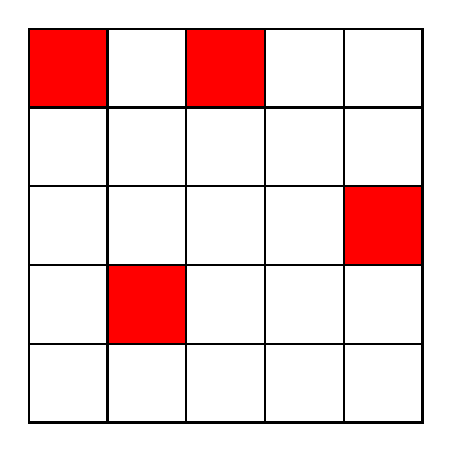
\begin{tikzpicture}
    [%%%%%%%%%%%%%%%%%%%%%%%%%%%%%%
        box/.style={rectangle,draw=black,thick, minimum size=1cm},
    ]%%%%%%%%%%%%%%%%%%%%%%%%%%%%%%

\foreach \x in {0,1,...,4}{
    \foreach \y in {0,1,...,4}
        \node[box] at (\x,\y){};
}
 
\node[box,fill=red  ] at (0,4){};  
\node[box,fill=red ] at (2,4){};  
\node[box,fill=red ] at (1,1){}; 
\node[box,fill=red ] at (4,2){}; 
\end{tikzpicture}
\end{minipage}
\caption[Pixel cluster selection algorithm]{The figure shows a representation of the pixel modules, \textit{left}: four hits (red) on four neighbouring pixels, these is considered a pixel cluster by the clustering algorithm. \textit{right}: the hits activate random pixel in the module, these will not be considered as a cluster by the clustering algorithm.}
\label{pixclust}
\end{figure}
A hit occurs when a charged particle passes through a silicon pixel, depositing an amount of energy in the pixel. The PCC method takes advantage of the high densities of pixels, and the relative low occupancy of the CMS tracker, to provide precise luminosity measurements, with good stable measurements over time. The number of pixel clusters activated, per bunch crossing, is a linear function of the number of proton-proton interactions per bunch crossing (pileup). During several zero-bias events, where the only requirement is that the bunches pass through one another on the interaction point, a mean number of pixel clusters, $\left\langle N_{\text {cluster }}\right\rangle
$,is activated:
\begin{equation}
\left\langle N_{\text {cluster }}\right\rangle\equiv\left\langle N_{\text {cluster/int}}\right\rangle\mu
\label{pcc}
\end{equation}
where $\left\langle N_{\text {cluster/int}}\right\rangle$ is the mean number of clusters activated per interaction and $\mu$ is the pileup. Using equation \ref{pileup} and \ref{pcc}, a calibration constant between the mean number of pixel cluster and the instantaneous luminosity can be defined:

\begin{equation}
    \left\langle N_{\text {cluster }}\right\rangle\equiv\frac{\sigma_{vis}}{f}\mathcal{L}_{ins}
\end{equation}
where the calibration constant, $\sigma_{vis}$, is   
\begin{equation}
    \sigma_{vis}=\sigma_{tot}\left\langle N_{\text {cluster/int}}\right\rangle
\end{equation}
The value of $\sigma_{vis}$ is determined using a van der Meer (vdM) scan, with 
\begin{equation}
    \sigma_{vis}= \frac{\left\langle N_{\text {cluster/vdM }}\right\rangle f }{\mathcal{L}_{ins/vdM}}
\end{equation}
where $\left\langle N_{\text {cluster/vdmM }}\right\rangle$ is the mean number of pixel cluster at the peak of the scan and $\mathcal{L}_{ins/vdM}$ is the instantaneous luminosity obtained in the scan \cite{CMS-PAS-LUM-12-001}.


%%%%%%%%%%%%%%%%%%%%%%%%%%%%%%%%%%%%%%%%%%%%%%%%%%%%%%%%%%%%%%%%%%%%%%%%%%%%%%%%%%%%%%%%%
\section{Cluster coincidence algorithm }

The other object used by the TEPX luminometer to measure the event rate are two-fold coincidences. Coincidences are less prone to contamination by false hits produced in the detector after a bunch crossing (afterglow), due to the slow dissipation of charge and neutrons produced by the surrounding material (albedo). Two-fold coincidences are created when a particle hits overlapping modules, in the different layers of the TEPX disks. Due to this, coincidences are more likely to be a real hit than random electrical noise. The cylinder/disk like geometry of the TEPX detector allows for coincidences to be constructed in two ways: coincidences in $\phi$ require modules overlapping in the same ring, in front and in the back of a double sided disk, while coincidences in $r$ requires overlapping modules from different layers. These two ways of constructing two-fold coincidences are illustrated in Figure \ref{3x2x}. The surface area of overlapping modules tends to be larger in $\phi$ than in the $r$ direction. In order for a 2x coincidence to be considered, activated pixel clusters must fall in to specific cuts (on their $\delta r$ and $\delta \phi$ separations). Finally, three-fold coincidences can occur as well, however, these types of coincidences are beyond the scope of this work.\\
Coincidences provide another method of measuring luminosity and bring more stability, linearity and precision to the TEPX luminometers.
\begin{center}
\begin{figure}[H]
    \centering
    \includegraphics[scale=.4]{Chapter3/3x2x.png}
    \caption[Regions where two-fold coincidences can occur in r and $\phi$.  ]{Diagram of the regions in r and $\phi$ where pixel modules overlap, between the front and the back layers of one double-sided disk, from which two-fold coincidences come. }
    \label{3x2x}
\end{figure}
\end{center}

%%%%%%%%%%%%%%%%%%%%%%%%%%%%%%%%%%%%%%%%%%%%%%%%%%%%%%%%%%%%%%%%%%%%%%%%%%%%%%%%%%%%%%%%%%

\section{Calibration using the van der Meer method }
The calibration of the luminometrs is done by performing van der Meer scans, where the goal is to determine the calibration constant $\sigma_{\text {vis}}$.\\
In practice, the normalized bunch transverse distributions of each beam is not known, thus the overlap width integrals in \ref{lumy2} cannot be solved analytically. The vdM scans determines the valued of these integrals by separating the two beams and moving them across each other while measuring the resulting rates (Figure \ref{vdm1} (left) illustrates this process)
\begin{equation}
    \int \rho_1(x)\rho_{2}(x)dx=\frac{R_{x}(0)}{\int R_{x}(\Delta x)d\Delta x}
\end{equation}
where $R_{x}(\Delta x)$ is the measured rate, when the beams are separated a distance $\Delta x$. Defining the beam overlap  width as
\begin{equation}
\Sigma_{x}=\frac{1}{\sqrt{2\pi}}\frac{\int R_{x}(\Delta x) d\Delta x}{R_{x}(0)}
\label{sigma2}
\end{equation}
doing the same can be done for $\Sigma_{y}$, equation \ref{lumy2} can be rewritten: 
\begin{equation}
    \mathcal{L}=\frac{N_1N_2N_p f}{2\pi\Sigma_x\Sigma_y}
\end{equation}
Once measurements have been taken, the rate is plotted as a function of beam separation and a Gaussian-like function is fitted to the data, as shown id Figure \ref{vdm1} (right). Using this function, the integral in equation \ref{sigma2} can be solved and the overlap width determined. Using \ref{lumy0} and \ref{lumy2} the calibration constant $\sigma_{vis}$ can be determined:
\begin{equation}
    \sigma_{vis}=\frac{2\pi \Sigma_x\Sigma_y}{N_1N_2N_p f} R_{peak}
    \label{sigmavis}
\end{equation}
where $R_{peak}$ is the measured rate at the peak of the scan \cite{CMS-PAS-LUM-18-002}\cite{CMS-PAS-LUM-12-001}. The original procedure can be found in \cite{vanderMeer:296752}.
\newcommand\gauss[2]{1/(#2*sqrt(2*pi))*exp(-((x-#1)^2)/(2*#2^2))} % Gauss function, parameters mu and sigma

\begin{figure}[ht]
\begin{minipage}[b]{0.5\linewidth}
\centering
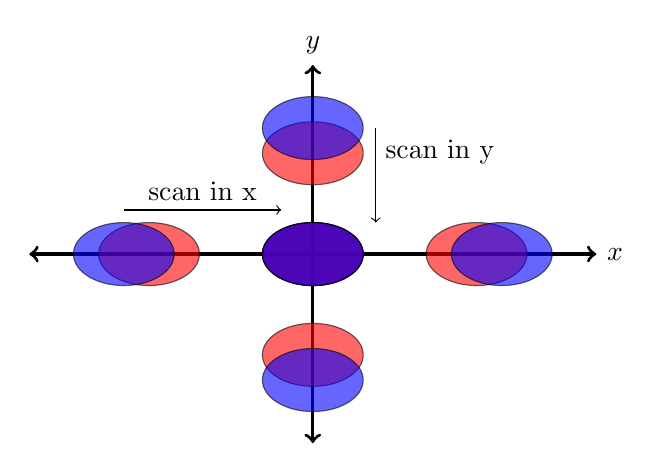
\begin{tikzpicture}[x=.5cm,y=.5cm, scale=1.6]

\draw[<->,very thick] (-4.5,0) -- (4.5,0)node[right] {$x$};
\draw[<->,very thick] (0,-3) -- (0,3) node[above] {$ y$};

%%%%%%%%%%%%%%%%%%%%%%%%%%%%%%%%%%%%%%%%%%%%%%%%%%%%%%%%%%%%%%%%%%%%%%%%%%%%%%%%%

\draw[fill=red, opacity=0.6] (0,-1.6) ellipse (4 mm and 2.5 mm);
\draw[fill=blue, opacity=0.6] (0,-2) ellipse (4 mm and 2.5 mm);


\draw[fill=red, opacity=0.6] (0,0) ellipse (4 mm and 2.5 mm);
\draw[fill=blue, opacity=0.6] (0,0) ellipse (4 mm and 2.5 mm);



\draw[fill=red, opacity=0.6] (0,1.6) ellipse (4 mm and 2.5 mm);
\draw[fill=blue, opacity=0.6] (0,2) ellipse (4 mm and 2.5 mm);


%%%%%%%%%%%%%%%%%%%%%%%%%%%%%%%%%%%%%%%%%%%%%%%%%%%%%%%%%%%%%%%%%%%%%%%%%%%
\draw[fill=red, opacity=0.6] (-2.6,0) ellipse (4 mm and 2.5 mm);
\draw[fill=blue, opacity=0.6] (-3,0) ellipse (4 mm and 2.5 mm);




\draw[fill=red, opacity=0.6] (0,0) ellipse (4 mm and 2.5 mm);
\draw[fill=blue, opacity=0.6] (0,0) ellipse (4 mm and 2.5 mm);



\draw[fill=red, opacity=0.6] (2.6,0) ellipse (4 mm and 2.5 mm);
\draw[fill=blue, opacity=0.6] (3,0) ellipse (4 mm and 2.5 mm);
%%%%%%%%%%%%%%%%%%%%%%%%%%%%%%%%%%%%%%%%%%%%%%%%%%%%%%%%%%%%%%%%%%%%%%%%%%%%%%%%%%%%%%%%%%%%%%
\draw[->,]  (1,2) -- (1,0.5)node[pos=0.25, right] {\text {scan in y}};
\draw[->,]  (-3,.7) -- (-0.5,.7)node[pos=0.5, above] {\text {scan in x}};
\end{tikzpicture}
\end{minipage}
%%%%%%%%%%%%%%%%%%%%%%%%%%%%%%%%%%%%%%%%%%%%%%%%%%%%%%%%%%%%%%%%%%%%%%%%%%%%%%%%%%%%%%%%%%%%%%%%%%%%%%%%%%%%%%%%%%%%%%%%%%%%%%%%%%%%%%%%%%%%%%%%%%%%%%%%%%%%%%%%%
\begin{minipage}[b]{0.5\linewidth}
\centering
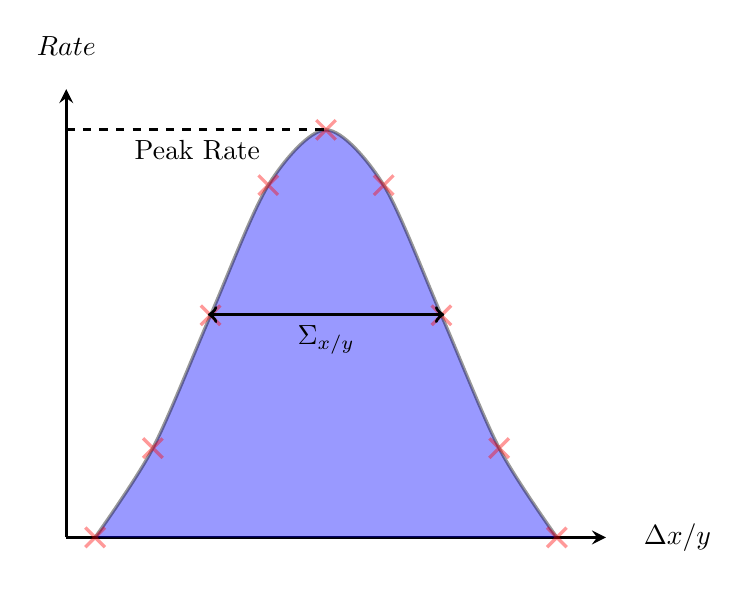
\begin{tikzpicture}
\begin{axis}[every axis plot post/.append style={ color=black,
  mark=x ,domain=-4:4,samples=9,smooth,fill=blue,opacity=0.4, mark size=5pt,mark options={color=red}}, % All plots: from -2:2, 50 samples, smooth, no marks
axis x  line=bottom,very thick, % no box around the plot, only x and y axis
axis y line=left,very thick, % the * suppresses the arrow tips
enlargelimits=upper, xmin=-4.5,
xlabel=\(\Delta x/y\),
ylabel=\(Rate\),
ytick={5},xtick={5},
every axis y label/.style={
    at={(ticklabel* cs:1.05)},
    anchor=south,
},
every axis x label/.style={
    at={(ticklabel* cs:1.05)},
    anchor=west,
},] % extend the axes a bit to the right and top
\addplot[]  {\gauss{0}{2}};


\end{axis}
\draw[<->,very thick] (1.8,2.83) -- (4.8,2.83)node[pos=0.5,below] {$\Sigma_{x/y}$};
\draw[dashed,very thick] (0,5.18) -- (3.33,5.18)node[pos=0.5,below] {\text {Peak Rate}};
\end{tikzpicture}

\end{minipage}
\caption[vdM scan process.]{\textit{Left}: A diagram that shows how the two beams are scanned across the x and y axis. \textit{ Right}: An example of a Gaussian-like function (Blue), being fitted to the rate measurements (red xs) taken during a VDM scan.}
\label{vdm1}
\end{figure}


%%%%%%%%%%%%%%%%%%%%%%%%%%%%%%%%%%%%%%%%%%%%%%%%%%%%%%%%%%%%%%%%%%%%%%%%%%%%%%%%
\section{Data acquisition}
After event rate measurements have been taken, the data needs to be safely transferred and stored. In order to do this, several systems are put in place. Every subdetector has a dedicated CMS subsystem or a dedicated BRIL (Beam Radiation, Instrumentation, and Luminosity) system that takes care of this process. In the case of the TEPX, and other luminometers described in section 3.4.1, a combination of CMS and BRIL systems will be used, while TEPXD4R1 will be solely operated by BRIL.\\
The way counts per bunch crossing measured by a given luminometer are stored in CMS, is by using histograms. Every time a full orbit of bunches collides (3564 bunches), the counts per bunch crossing is histogramed and stored. Depending on the geometry of the subdetector, the number of histograms generated by each changes. In the case of TEPX and TEPXD4R1 a histogram is created per quarter ring, this means that a total of 152 histograms are created by TEPX (not including the histograms from D4R1) and 8 by TEPXD4R1, in one orbit. The histograming is done by the dedicated back-end of each subdetector, a combination of software and hardware components in charge of creating these histograms. Once the histograms have been correctly created they are read, processed and stored by the BRILDAQ (BRIL data acquisition) system. Figure \ref{histhit} shows an example of a histograms for TEPX in the case of pixel clusters.
\begin{center}
    \begin{figure}[H]
        \centering
        \includegraphics[scale=0.5]{Chapter3/histbx.png}
        \caption[Histogram of the mean number of pixel clusters per bunch crossing (BX) measured by the Phase-1 pixel detector.]{The histogram shows the mean number of pixel clusters per bunch crossing (BX) for one lumisection (23.3 seconds), measured by the Phase-1 pixel detector during regular physics runs. The measurements from the 2018 data taking period.}
        \label{histhit}
    \end{figure}
\end{center}
Once histograms have been created, safely transferring and storing them is important, in order to do this the memory required to store them needs to be known. The memory size of each histogram depends on the information in each of  them. All histograms have 3564 bins, one bin for each bunch crossing, these bins store the number of counts measured in a given bunch crossing, thus, the bits of information stored in these bins will give the memory of each histogram.
\begin{equation}
    \text {Memory per Hist}= \text {No. of Bins}\times \text {bits per Bin}
    \label{histm}
\end{equation}
 where the bits per Bin are calculated using 
 \begin{equation}
     \text {bits per Bin}= log_2(N)
     \label{logn}
 \end{equation}
where $N$ is the maximum expected number of counts per bunch crossing for a given integration period, it is worth mentioning that the results from equation \ref{logn} are rounded up to the closes integer. The maximum expected number of counts per bunch crossing is given by 

\begin{equation}
    N=n\frac{\text {Total Trigger Rate}}{3564}t
    \label{N}
\end{equation}
where $n$ is the mean number of counts per event and $t$ is the integration period. Equation \ref{N} assumes that the Total Trigger Rate is distributed uniformly. Once the memory of the histogram is known, the data bandwidth needed to store all the histograms can be calculated, the Data Transfer Rate is given by 
\begin{equation}
    \text {Data Transfer Rate}=\frac{No. Hist\times Memory per Hist}{t}
    \label{drate}
\end{equation}
where No. Hist is the number of histograms created by the detector and t is the time in which the information is transferred.\\

\subsection*{32-bit word implementation}
The data at CMS is not transferred bit by bit, rather, is transferred in packages of information called words. Each word contains 32-bits of information, this means that all data transferred has to, first, be converted in to a 32-bit word. The way this is applied to the histograms is by converting the information in each bin in to a word, this is done in two ways:
\begin{itemize}
    \item If the Bits per bin$\leq16$ bits, the number of bits is
rounded to 16 and two bins are grouped in one word.
\item If $16\leq$ Bits per bin$\leq32$,  the number of bits is
rounded to 32-bit word and one word is used for each bin.
\end{itemize}

Aside from this, the TEPX luminometers use additional words for the overhead of the histograms data format:
\begin{itemize}
    \item 9 words for the header for TEPX and D4R1.
    \item  768 words for errors for TEPX and 160 for D4R1.
    \item 4 words for the mask for TEPX and 2 forD4R1.
\end{itemize}
These additional data has to be taken in to account for each histograms, when calculating the needed memory to store and transfer them. Finally, using equation \ref{logn} the bits per bin can be calculated, using data from the high pileup simulation \cite{datarates}. The results for the TEPX luminometers is shown in Table \ref{bitsperbin}.
\begin{table}[ht]
\centering
\caption[ Memory bits required per histogram bin for the TEPX luminometers.]{Table shows the Trigger rate (kHz), counts per event per detector unit (histogram), number of counts per bx per integration period (1s) and the memory bits required per histogram bin.}
\scalebox{.7}{
\begin{tabular}{|l |c |c |c |c|}
\hline
&  Trigger rate (kHz) & Counts per event & Counts/bx/1s&Bits/bin\\
\hline
TEPXD4R1 Clusters&825&539&1.25e+05&17\\
\hline
TEPXD4R1 2x Coincidences&825&54&1.25e+04&14\\
\hline
TEPX Clusters&75&539&1.13e+04&14\\
\hline
TEPX 2x Coincidences&75&54&1.14e+03&11\\
\hline
\end{tabular}}
\label{bitsperbin}
\end{table}
Using this and equation \ref{drate}, the data rates can be calculated, the results are shown in Table \ref{dataratet} for a transferring time of 1 s.
\begin{table}[ht]
\centering
\caption[Data transfer rates for the TEPX luminometers.]{Data transfer rates for the TEPX luminometers for pileup 200. Columns shown are number of histograms, memory per histogram and data transfer rates (Mbps) for an integration period of 1s. }
\scalebox{.8}{

\begin{tabular}{|l  |c |c |c|}
\hline
&  Number of Histograms & Memory per histogram (Kb) & Data Transfer Rates (Mbps)\\
\hline
TEPXD4R1 Clusters&8&124&0.95\\
\hline
TEPXD4R1 2x Coincidences&8&67&0.5\\
\hline
TEPX Clusters&152&82&12.5\\
\hline
TEPX 2x Coincidences&152&82&12.5\\
\hline
\end{tabular}}
\label{dataratet}
\end{table}
%%%%%%%%%%%%%%%%%%%%%%%%%%%%%%%%%%%%%%%%%%%%%%%%%%%%%%%%%%%%%%%%%%%%%%%%%%%%%%%%%%%%%%%%%%%%%%%%%%%%%%%%%%%%%%%%%%%
\subsection{Other luminometers}

The TEPX luminometer is not the only luminometer of the CMS Phase-2 detector, each layer of the detector will have a dedicated luminometer, and corresponding algorithm, to ensure the best luminosity measurements possible.
Figure \ref{cmslum} shows the location of the different luminometers at the CMS detector, for the Phase-2 upgrade. A brief description of the luminometers is presented below.
\begin{center}
\begin{figure}[H]
    \centering
    \includegraphics[scale=0.3]{Chapter3/cmdlum.png}
    \caption[Different subsystems and luminometrs at CMS.]{Layout of the different subsystems and luminometrs at CMS. }
    \label{cmslum}
\end{figure}
\end{center}
\subsection*{Outer tracker layer 6}
From the outer tracker (OT), layer 6 will be a designated luminometer. The object used by these luminometer are track stubs, which are two-hit coincidences between closely spaced silicon modules. Figure \ref{ot} show the layout of the new Phase-2 outer tracker, layer 6 is located in the outer tracker barrel, specifically, the TB2S section.
\begin{center}
\begin{figure}[H]
    \centering
    \includegraphics[scale=.4]{Chapter3/ot.png}
    \caption[Outter tracker layout.]{Diagram of the different parts that conform the outer tracker, the two barrel regions, TBPS and TB2S, and the end-cap region TEDD. The OT layer 6 luminometer corresponds to the last upper layer of TB2S. }
    \label{ot}
\end{figure}
\end{center}

Layer 6 consists of 76 ladders of 12 strip modules made of two Si-strip sensors, as shown in Figure \ref{otlather} (left). The ladders span fully, in the azimuthal range, at each end of the CMS detector. The reconstruction method of the track stubs is shown in Figure \ref{otlather} (right) as well. The tracks are reconstructed at 40 MHz.
\begin{center}
\begin{figure}[H]
    \centering
    \includegraphics[scale=.7]{Chapter3/otlather.PNG}
    \caption[Example of an OT layer 6 ladder and the stub selection process.]{\textit{Left}: An example of a ladder with the the 12 strip modules (regions in yellow). \textit{Right}: Diagram of the stub selection process. The black squares represent hits, and the green squares represent the regions where the other hit could take place, to be considered a stub.}
    \label{otlather}
\end{figure}
\end{center}

The OT layer 6 luminometers, creates one histograms per one 12 module ladder, for a total of 152. As well as the TEPX luminometers, the histograms created in layer 6 will have additional words for the overhead of the histograms data format:
\begin{itemize}
    \item 9 words for the header.
    \item  192 words for errors.
    \item 4 words for the mask.
\end{itemize}

Figure \ref{otstubs} shows the expected number of track stubs per bunch crossing as function of the ladders ID. Tables 3.3
and 3.4 show the expected Bits per Bin and the Data Transfer Rates for the OT layer 6 luminometer, calculated using data from the high pileup simulation.
\begin{center}
\begin{figure}[H]
    \centering
    \includegraphics[scale=.4]{Chapter3/OT-Rates.png}
    \caption[Simulated expected number of stubs per ladder per event.]{Simulated expected number of stubs per ladder per event as a function of ladder ID.}
    \label{otstubs}
\end{figure}
\end{center}
%%%%%%%%%%%%%%%%%%%%%%%%%%%%%%%%%%%%%%%%%%%%%%%%%%%%%%%%%%%%%%%%%%%%%%%%%%%%%%%%%
\subsection*{Muon drift tube}
The muon DT luminometer follows the same design described in section 2.2. The entire DT system is formed by 250 gas chambers, installed in the barrel yoke of the CMS detector, as shown in Figure \ref{Muons}. The chambers are distributed across 5 wheels labeled YB0, YB$\pm1$ and YB$\pm2$, four radial stations, MB1-MB4, and 12 $\phi$ sectors \cite{ABBIENDI2009192}.

The objects used by this luminometer are called trigger primitives, which are reconstructed muon track segments per DT chamber. The tracks are reconstructed at a trigger frequency of  40 $MHz$,  using hits from the DT and RPC detectors. The rate of trigger primitives has being studied and extrapolated to the expected  instantaneous luminosity of the HL-LHC, $7.5\times 10^{34}$ $cm^{-2}s^{-1}$, using  the data from Run 2. Figure \ref{dtrate} shows the expected rates for the YB0 and YB+2 wheels. The large difference on the measured rate, between the MB1 and the rest of the chambers in the MB2 and MB3 stations, is due to a significant contribution of particle from punch-through jets.
\begin{figure}[H]
\centering
\includegraphics[width=.48\textwidth]{Chapter3/DT_Trigger_extraploation_YB.pdf}
\includegraphics[width=.48\textwidth]{Chapter3/DT_Trigger_extraploation_YBp2.pdf}
\caption[Expected rates of trigger primitives per DT chamber]{Expected rates of trigger primitives per DT chamber for the YB0 (left) and YB+2 (right) wheels.}
\label{dtrate}
\end{figure}
The DT luminometer will create one histogram per DT chamber, giving a total of 250 histograms. Tables \ref{bitsperbinall} and \ref{dataratesall} show the expected Bits per Bin and the  Data Transfer Rates for the DT luminometer, using extrapolated data from the 2018 data taking period.
%%%%%%%%%%%%%%%%%%%%%%%%%%%%%%%%%%%%%%%%%%%%%%%%%%%%%%%%%%%%%%%%%%%%%%%%%%%%%%%%
\subsection*{BMTF }
The Barrel Muon Track Finder (BMTF) is an algorithm that uses reconstructed muon tracks to provide luminosity measurements. As its name suggests, The algorithm uses information from all the DT and RPC gas chambers, located in the barrel of the muon system, to reconstruct muon tracks.
One histograms is created by the algorithm. Tables \ref{bitsperbinall} and \ref{dataratesall} show the expected Bits per Bin and the  Data Transfer Rates for the BMTF algorithm \cite{Bachtis:2648953}. As well as the DT luminometer, BTMS uses  extrapolated data from the 2018 data taking period.
%%%%%%%%%%%%%%%%%%%%%%%%%%%%%%%%%%%%%%%%%%%%%%%%%%%%%%%%%%%%%%%%
\subsection{Data transfer rates for all luminometers}
Using the number of histograms, as well as the mean number of counts per event for each luminometer \cite{datarates}, the number of Bits per Bin as well as the Data Transfer Rates can be calculated for all luminometers. This is shown is Tables \ref{bitsperbinall} and \ref{dataratesall} respectively.
\begin{table}[H]
\centering
\caption[Memory bits required per histogram bin for all luminometers.]{Triger rate (kHz), counts per event per detector unit (histogram), number of counts per bx per integration period (1s) and the memory bits required per histogram bin.}
\scalebox{.7}{
\begin{tabular}{|l |c |c |c |c|}
\hline
&  Trigger rate (kHz) & Counts per event & Counts/bx/1s&Bits/bin\\
\hline
TEPXD4R1 Clusters&825&539&1.25e+05&17\\
\hline
TEPXD4R1 2x Coincidences&825&54&1.25e+04&14\\
\hline
TEPX Clusters&75&539&1.13e+04&14\\
\hline
TEPX 2x Coincidences&75&54&1.14e+03&11\\
\hline
OT Layer 6 track stubs&40000&8&8.98e+04&17\\
\hline
DT Trigger Primitives&40000&0.0125&140&8\\
\hline
BMTF Tracks&40000&0.041&460&9\\
\hline
\end{tabular}}
\label{bitsperbinall}
\end{table}
\begin{table}[H]
\centering
\caption[Data transfer rates for the different luminometers.]{Data transfer rates for the different luminometers for pileup 200. Columns shown are number of histograms, memory per histogram and data transfer rates (Mbps) for an integration period of 1s. }
\scalebox{.8}{
\begin{tabular}{|l  |c |c |c|}
\hline
&  Number of Histograms & Memory per histogram (Kb) & Data Transfer Rates (Mbps)\\
\hline
TEPXD4R1 Clusters&8&124&0.95\\
\hline
TEPXD4R1 2x Coincidences&8&67&0.5\\
\hline
TEPX Clusters&152&82&12.5\\
\hline
TEPX 2x Coincidences&152&82&12.5\\
\hline
OT Layer 6 track stubs&152&120&18.3\\
\hline
DT Trigger Primitives&250&28&7.13\\
\hline
BMTF Track&1&57&0.057\\
\hline
\end{tabular}}
\label{dataratesall}
\end{table}

From these tables it can be concluded that the minimum bandwidth required will be 18.3 Mbps, corresponding to the OT luminometer. The total storage needed per day for all luminometers presented here can be calculated, assuming an operation time of 12 hours, the total storage needed will be 280.46 GB. Since other luminometers will be in operation, besides the ones discussed here, 280.46 GB is the minimum storage per day required to ensure no data is lost.